\documentclass[11pt, a4paper]{article}
\usepackage[a4paper, margin=2.5cm]{geometry}
\usepackage[utf8]{inputenc}
\usepackage[T1]{fontenc}
\usepackage[spanish,es-nodecimaldot]{babel}
\usepackage{enumitem}
\setlist[itemize]{label=-}
\usepackage{amsmath}
\usepackage{amssymb}
\usepackage{booktabs}
\usepackage{graphicx}
\usepackage{xcolor}
\usepackage{listings}
\usepackage{hyperref}
\usepackage{float}
\usepackage{caption}

\makeatletter
\setlength{\@fptop}{0pt}
\setlength{\@fpbot}{0pt plus 1fil}
\makeatother

\lstset{
    language=Matlab,
    backgroundcolor=\color{gray!6},
    basicstyle=\ttfamily\footnotesize,
    keywordstyle=\color{blue}\bfseries,
    commentstyle=\color{green!50!black}\itshape,
    stringstyle=\color{purple},
    numbers=left,
    numberstyle=\tiny\color{gray},
    stepnumber=1,
    numbersep=8pt,
    frame=single,
    rulecolor=\color{gray!30},
    tabsize=4,
    showspaces=false,
    showstringspaces=false,
    breaklines=true,
    breakatwhitespace=true,
    literate={á}{{\'a}}1 {é}{{\'e}}1 {í}{{\'i}}1 {ó}{{\'o}}1 {ú}{{\'u}}1 {ñ}{{\~n}}1 {Á}{{\'A}}1 {É}{{\'E}}1 {Í}{{\'I}}1 {Ó}{{\'O}}1 {Ú}{{\'U}}1 {Ñ}{{\~N}}1
}

\hypersetup{
    colorlinks=true,
    linkcolor=blue!70!black,
    citecolor=blue!70!black,
    urlcolor=blue!70!black
}

\title{\textbf{Segundo Trabajo Grupal: Simulación de Colas}\\[0.3em]
\large Herramientas Matemáticas para el Manejo de la Información -- 2026-3\\[0.2em]
\normalsize Modelo Asignado: Sistema de Espera Erlang C ($M/M/k/\infty/\infty$)}
\author{David Stiven Muñoz Amaya -- 20202020071\\[0.2em]
\textit{Facultad de Ingeniería, Universidad Distrital Francisco José de Caldas}}
\date{Noviembre de 2026}

\begin{document}

\maketitle

\begin{abstract}
El presente documento constituye el informe técnico y experimental del segundo trabajo grupal de la asignatura Herramientas Matemáticas para el Manejo de la Información. Se aborda en detalle el diseño, formalización analítica y desarrollo de una herramienta computacional en MATLAB para la simulación de colas bajo el modelo Erlang C ($M/M/k/\infty/\infty$). En las primeras tres secciones se expone el modelo matemático riguroso (diagrama de estados, balance de flujo, deducción de la probabilidad de espera y tiempo medio de espera $E[T_w]$), el diseño del algoritmo de simulación multi-servidor orientado a eventos temporales y la validación cruzada experimental vs. analítica bajo variaciones sistemáticas de la intensidad de tráfico ofrecido $A = \lambda/\mu$. Finalmente, se presenta la estructura formal y metodológica reservada para la incorporación de generadores empíricos basados en cuantiles (`superfuncion`), la evaluación de arribos no exponenciales y el dimensionamiento de un caso de estudio real en ingeniería.
\end{abstract}

\vspace{0.5em}
\noindent\textbf{Palabras clave:} Teoría de colas, modelo Erlang C, simulación por eventos, tiempo medio de espera, intensidad de tráfico, procesos de Markov.

\vspace{1em}
\hrule
\vspace{1em}

\section{Actividad 1: Modelo Matemático de la Cola ($M/M/k/\infty/\infty$)}

\subsection{Definición del Sistema y Espacio de Estados}
El modelo asignado al grupo corresponde al sistema de colas multicanal sin pérdidas con capacidad de espera infinita, formalizado según la notación de Kendall como $M/M/k/\infty/\infty$ o modelo de retardo de Erlang (Erlang C). Las características fundamentales del sistema son:
\begin{itemize}
    \item \textbf{Proceso de arribo ($M$):} Los clientes arriban al sistema según un proceso de Poisson homogéneo con tasa constante $\lambda$. En consecuencia, los tiempos entre arribos consecutivos se distribuyen exponencialmente con parámetro $\lambda$, es decir, con media $1/\lambda$.
    \item \textbf{Proceso de atención ($M$):} Cada uno de los $k$ servidores en paralelo atiende clientes de forma estadísticamente independiente, con tiempos de servicio distribuidos exponencialmente de parámetro $\mu$ (media $1/\mu$).
    \item \textbf{Servidores en paralelo ($k$):} Existen $k$ servidores idénticos que operan en simultáneo ($k \in \mathbb{Z}^+$).
    \item \textbf{Disciplina de servicio y capacidad de almacenamiento ($\infty/\infty$):} La cola posee capacidad ilimitada (no hay bloqueo ni rechazo; los usuarios esperan hasta ser atendidos). La disciplina de atención es FIFO (\textit{First In, First Out}).
\end{itemize}

El estado del sistema en un instante de tiempo $t$, denotado por $N(t) = n \in \{0, 1, 2, \dots\}$, representa el número total de clientes presentes en el sistema (tanto los que están siendo atendidos como los que esperan en cola).

\subsection{Diagrama de Transición de Estados}
Las tasas de nacimiento ($\lambda_n$) y de muerte ($\mu_n$) entre estados contiguos son:
\begin{equation}
\lambda_n = \lambda, \quad \forall n \ge 0
\end{equation}
\begin{equation}
\mu_n = 
\begin{cases} 
n\mu, & \text{si } 0 \le n < k \quad (\text{sólo } n \text{ servidores activos}) \\
k\mu, & \text{si } n \ge k \quad (\text{todos los } k \text{ servidores activos})
\end{cases}
\end{equation}

En la Figura \ref{fig:diagrama_erlang_c} se observa la cadena de Markov en tiempo continuo correspondiente a este proceso de nacimiento y muerte.

\begin{figure}[H]
    \centering
    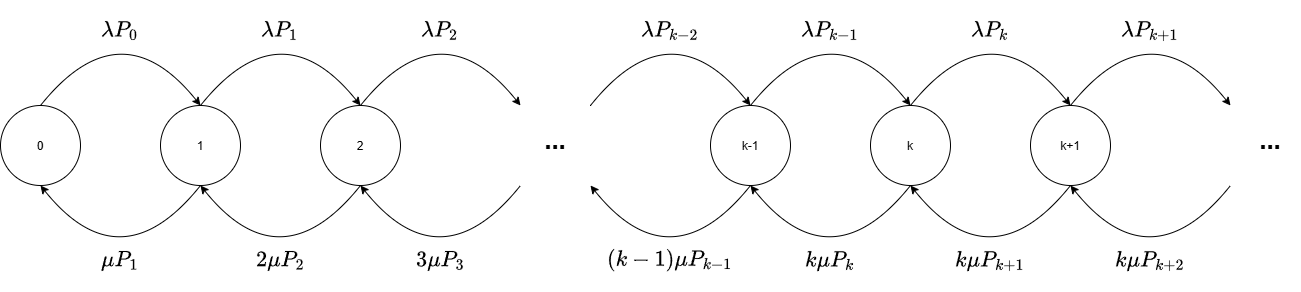
\includegraphics[width=0.88\textwidth]{Erlang_C_Diagram.drawio.png}
    \caption{Diagrama de transición de estados para el modelo de espera Erlang C ($M/M/k/\infty$).}
    \label{fig:diagrama_erlang_c}
\end{figure}

\subsection{Ecuaciones de Estado Estacionario (Balance de Flujo)}
Bajo la condición de estabilidad $A < k$, donde $A = \lambda/\mu$ representa el tráfico ofrecido en Erlangs, el sistema alcanza un régimen permanente o estacionario donde la tasa promedio de entrada a cada estado es idéntica a la tasa promedio de salida:
\begin{table}[H]
\centering
\renewcommand{\arraystretch}{1.35}
\resizebox{\textwidth}{!}{%
\begin{tabular}{@{}ccccc@{}}
\toprule
\textbf{Estado} & \textbf{Tasa de salida} & $=$ & \textbf{Tasa de llegada} & \textbf{Despeje} \\ 
\midrule
$0$ & $\lambda P_0$ & $=$ & $\mu P_1$ & $P_1 = \dfrac{\lambda}{\mu} P_0$ \\[0.5em]
$1$ & $\mu P_1 + \lambda P_1$ & $=$ & $\lambda P_0 + 2\mu P_2$ & $P_2 = \dfrac{\lambda}{2\mu} P_1$ \\[0.5em]
$2$ & $2\mu P_2 + \lambda P_2$ & $=$ & $\lambda P_1 + 3\mu P_3$ & $P_3 = \dfrac{\lambda}{3\mu} P_2$ \\[0.5em]
$\vdots$ & $\vdots$ & & $\vdots$ & $\vdots$ \\[0.5em]
$k - 1$ & $(k-1)\mu P_{k-1} + \lambda P_{k-1}$ & $=$ & $\lambda P_{k-2} + k\mu P_k$ & $P_k = \dfrac{\lambda}{k\mu} P_{k-1}$ \\[0.5em]
$k$ & $k\mu P_k + \lambda P_k$ & $=$ & $\lambda P_{k-1} + k\mu P_{k+1}$ & $P_{k+1} = \dfrac{\lambda}{k\mu} P_k$ \\[0.5em]
$k + 1$ & $k\mu P_{k+1} + \lambda P_{k+1}$ & $=$ & $\lambda P_k + k\mu P_{k+2}$ & $P_{k+2} = \dfrac{\lambda}{k\mu} P_{k+1}$ \\[0.5em]
\bottomrule
\end{tabular}%
}
\caption{Ecuaciones de estado estacionario (tasa de salida $=$ tasa de llegada) y relaciones de recurrencia.}
\label{tab:balance_estados}
\end{table}

\subsection[Calcular Pn en función de P0]{Calcular $P_n$ en función de $P_0$}

Para los primeros estados se tiene la relación general:
\[
P_n = \frac{1}{n!} \left( \frac{\lambda}{\mu} \right)^n P_0
\]

Como a partir de $k$ servidores la tasa ya no aumenta sino que queda fija en $k\mu$, se analiza en 2 casos (donde $n-k$ representa la distancia que hay entre $k$ y $n$):

\[
P_n = 
\begin{cases} 
\displaystyle \frac{1}{n!} \left( \frac{\lambda}{\mu} \right)^n P_0, & \text{si } 0 \le n < k \\[1.5em]
\displaystyle \frac{1}{k! \, k^{n-k}} \left( \frac{\lambda}{\mu} \right)^n P_0, & \text{si } n \ge k 
\end{cases}
\]

\subsection[Pn en función de los parámetros lambda y mu]{$P_n$ en función de los parámetros $\lambda$ y $\mu$}

Por condición de normalización:
\[
P_0 + P_1 + P_2 + \dots = 1 \implies \sum_{n=0}^{\infty} P_n = 1
\]

Separando la sumatoria en los dos casos:
\[
\sum_{n=0}^{k-1} P_n + \sum_{n=k}^{\infty} P_n = 1
\]

Sustituyendo las expresiones de $P_n$ en función de $P_0$:
\[
\sum_{n=0}^{k-1} \left[ \frac{1}{n!} \left( \frac{\lambda}{\mu} \right)^n P_0 \right] + \sum_{n=k}^{\infty} \left[ \frac{1}{k! \, k^{n-k}} \left( \frac{\lambda}{\mu} \right)^n P_0 \right] = 1
\]

Factorizando $P_0$:
\[
P_0 \left( \sum_{n=0}^{k-1} \frac{1}{n!} \left( \frac{\lambda}{\mu} \right)^n + \sum_{n=k}^{\infty} \frac{1}{k! \, k^{n-k}} \left( \frac{\lambda}{\mu} \right)^n \right) = 1
\]

Desarrollando la segunda sumatoria:
\[
\sum_{n=k}^{\infty} \frac{1}{k! \, k^{n-k}} \left( \frac{\lambda}{\mu} \right)^n = \frac{1}{k!} \left( \frac{\lambda}{\mu} \right)^k \sum_{n=k}^{\infty} \left( \frac{\lambda}{k\mu} \right)^{n-k}
\]

Haciendo el cambio de variable $m = n - k$ (cuando $n = k \to m = 0$):
\[
= \frac{1}{k!} \left( \frac{\lambda}{\mu} \right)^k \sum_{m=0}^{\infty} \left( \frac{\lambda}{k\mu} \right)^m
\]

Definiendo $A = \frac{\lambda}{k\mu}$, dado que $|A| < 1$ (para que la serie geométrica converja, es decir, $\lambda < k\mu$):

\[
\sum_{m=0}^{\infty} A^m = \frac{1}{1 - A} = \frac{1}{1 - \frac{\lambda}{k\mu}} = \frac{k\mu}{k\mu - \lambda}
\]

Por lo tanto, el segundo término resulta en:
\[
= \frac{1}{k!} \left( \frac{\lambda}{\mu} \right)^k \left( \frac{k\mu}{k\mu - \lambda} \right)
\]

Sustituyendo en la ecuación con $P_0$ factorizado y despejando $P_0$:
\begin{equation}
P_0 = \left[ \sum_{n=0}^{k-1} \frac{1}{n!} \left( \frac{\lambda}{\mu} \right)^n + \frac{1}{k!} \left( \frac{\lambda}{\mu} \right)^k \left( \frac{k\mu}{k\mu - \lambda} \right) \right]^{-1}
\label{eq:P0_final}
\end{equation}

Finalmente, reemplazando $P_0$ en la expresión por partes de $P_n$:

\begin{equation}
P_n = 
\begin{cases} 
\displaystyle \frac{1}{n!} \left( \frac{\lambda}{\mu} \right)^n \left[ \sum_{i=0}^{k-1} \frac{1}{i!} \left( \frac{\lambda}{\mu} \right)^i + \frac{1}{k!} \left( \frac{\lambda}{\mu} \right)^k \left( \frac{k\mu}{k\mu - \lambda} \right) \right]^{-1}, & \text{si } 0 \le n < k \\[2em]
\displaystyle \frac{1}{k! \, k^{n-k}} \left( \frac{\lambda}{\mu} \right)^n \left[ \sum_{i=0}^{k-1} \frac{1}{i!} \left( \frac{\lambda}{\mu} \right)^i + \frac{1}{k!} \left( \frac{\lambda}{\mu} \right)^k \left( \frac{k\mu}{k\mu - \lambda} \right) \right]^{-1}, & \text{si } n \ge k 
\end{cases}
\label{eq:Pn_final}
\end{equation}

Nótese que definiendo la intensidad de tráfico ofrecido como $A = \frac{\lambda}{\mu}$, el factor de la serie geométrica se expresa de manera compacta como $\frac{k\mu}{k\mu - \lambda} = \frac{k}{k - A}$, bajo la condición de estabilidad del sistema $A < k$.

\subsection[Medida de Desempeño: Probabilidad de Espera y Tiempo Medio E[Tw]]{Medida de Desempeño: Probabilidad de Espera y Tiempo Medio $E[T_w]$}

\subsubsection{Interpretación conceptual}

Los sistemas Erlang B ($M/M/k/k$, con pérdida) y Erlang C ($M/M/k/\infty$, con espera) se comportan de forma idéntica mientras existan servidores libres ($0 \le n < k$), ya que la tasa de llegada es $\lambda$ y la de servicio es $n\mu$. Por ello, ambos comparten los mismos términos proporcionales $\frac{A^n}{n!}$, donde $A = \frac{\lambda}{\mu}$ es el tráfico ofrecido.

La diferencia ocurre al alcanzar el límite de $k$ servidores ocupados:
\begin{itemize}
    \item \textbf{En Erlang B:} El sistema se trunca en $n = k$. Todo cliente que llega cuando $N = k$ es bloqueado y se pierde.
    \item \textbf{En Erlang C:} Si llegan más clientes ($n \ge k$), forman una fila infinita atendida a tasa constante $k\mu$. Al sumar las probabilidades de todos los estados de espera ($n \ge k$) mediante una serie geométrica (con $A < k$), aparece el factor de amplificación de la cola $\left(\frac{k}{k - A}\right)$ acompañando al término $\frac{A^k}{k!}$.
\end{itemize}

\subsubsection{Demostración matemática}

Para el sistema Erlang B, la probabilidad de bloqueo $E_{1,k}$ está dada por:
\[
E_{1,k} = \frac{\frac{A^k}{k!}}{\sum\limits_{n=0}^{k} \frac{A^n}{n!}}
\]

Separando el último término ($n = k$) de la sumatoria del denominador e invirtiendo la fracción:
\[
\frac{1}{E_{1,k}} = \frac{\sum\limits_{n=0}^{k-1} \frac{A^n}{n!} + \frac{A^k}{k!}}{\frac{A^k}{k!}} = \frac{\sum\limits_{n=0}^{k-1} \frac{A^n}{n!}}{\frac{A^k}{k!}} + 1
\]

Despejando el término de la sumatoria:
\begin{equation}
\frac{\sum\limits_{n=0}^{k-1} \frac{A^n}{n!}}{\frac{A^k}{k!}} = \frac{1}{E_{1,k}} - 1 = \frac{1 - E_{1,k}}{E_{1,k}}
\label{eq:sumatoria_erlangB}
\end{equation}

Por otro lado, para el sistema Erlang C ($M/M/k/\infty$), la probabilidad de espera se estructura como:
\[
E_{2,k} = P[T_w > 0] = \frac{A^k}{k!} \left( \frac{k}{k - A} \right) P_0
\]
donde la probabilidad de sistema vacío ($P_0$) viene dada por:
\[
P_0 = \left[ \sum\limits_{n=0}^{k-1} \frac{A^n}{n!} + \frac{A^k}{k!} \left( \frac{k}{k - A} \right) \right]^{-1}
\]
Al sustituir $P_0$ en la expresión de $E_{2,k}$, se obtiene la ecuación completa de Erlang C:
\[
E_{2,k} = \frac{\frac{A^k}{k!} \left(\frac{k}{k - A}\right)}{\sum\limits_{n=0}^{k-1} \frac{A^n}{n!} + \frac{A^k}{k!} \left(\frac{k}{k - A}\right)}
\]

Dividiendo el numerador y el denominador de la expresión de $E_{2,k}$ entre $\frac{A^k}{k!}$:
\[
E_{2,k} = \frac{\frac{k}{k - A}}{\frac{\sum\limits_{n=0}^{k-1} \frac{A^n}{n!}}{\frac{A^k}{k!}} + \frac{k}{k - A}}
\]

Sustituyendo la ecuación \eqref{eq:sumatoria_erlangB} en el denominador:
\[
E_{2,k} = \frac{\frac{k}{k - A}}{\left(\frac{1 - E_{1,k}}{E_{1,k}}\right) + \frac{k}{k - A}}
\]

Multiplicando el numerador y el denominador por $E_{1,k}(k - A)$ para simplificar las fracciones:
\[
E_{2,k} = \frac{k \cdot E_{1,k}}{(1 - E_{1,k})(k - A) + k \cdot E_{1,k}}
\]

Expandiendo el producto en el denominador y cancelando los términos $-k \cdot E_{1,k}$ y $+k \cdot E_{1,k}$:
\[
\text{Denominador} = k - A - k \cdot E_{1,k} + A \cdot E_{1,k} + k \cdot E_{1,k} = k - A + A \cdot E_{1,k}
\]

Factorizando $A$ en el denominador, se obtiene finalmente la ecuación de relación directa:
\begin{equation}
\mathbf{E_{2,k} = \frac{k \cdot E_{1,k}}{k - A + A \cdot E_{1,k}} = \frac{k \cdot E_{1,k}}{k - A(1 - E_{1,k})}}
\label{eq:erlangC_directa}
\end{equation}

Donde:
\begin{itemize}
    \item $E_{1,k}$: Probabilidad de bloqueo en Erlang B.
    \item $k$: Número de servidores ($k \in \mathbb{Z}^+$).
    \item $A$: Intensidad de tráfico ofrecido $A = \frac{\lambda}{\mu}$ (bajo condición de estabilidad $A < k$).
\end{itemize}

\subsubsection{Cálculo del Tiempo Medio de Espera $E[T_w]$}
Conocida la probabilidad de espera $P[T_w > 0] = E_{2,k}$, el tiempo medio de espera en cola $E[T_w]$ (medida de desempeño asignada al modelo Erlang C) se calcula analíticamente mediante:
\begin{equation}
E[T_w] = \frac{1}{\mu(k - A)} P[T_w > 0] = \frac{E_{2,k}}{\mu(k - A)}
\label{eq:ETw_teorico}
\end{equation}
Asimismo, las variables de interés complementarias del sistema quedan dadas por:
\begin{equation}
E[N_w] = \frac{A}{k - A} P[T_w > 0]
\end{equation}
\begin{equation}
E[N_s] = \frac{A}{k - A} P[T_w > 0] + A
\end{equation}
\begin{equation}
P[T_w > t] = P[T_w > 0] \, e^{-\mu(k - A)t}, \quad t \ge 0
\end{equation}

\vspace{1em}
\hrule
\vspace{1em}

\section{Actividad 2: Diseño y Codificación de la Función de Simulación en MATLAB}

\subsection{Lógica de Simulación Multi-Servidor por Eventos Discretos}

El algoritmo toma como variables de entrada dos vectores unidimensionales generados externamente:
\begin{itemize}
    \item \texttt{tea}: Vector con los tiempos entre arribos consecutivos.
    \item \texttt{tds}: Vector con los tiempos de servicio requeridos por cada cliente.
\end{itemize}

A partir de dichos vectores, se define un vector acumulativo que marca el instante exacto de arribo de cada usuario en la línea de tiempo global:
\begin{equation}
\text{\texttt{reloj}}(i) = \sum_{j=1}^{i} \text{\texttt{tea}}(j)
\end{equation}

Para gestionar los $k$ servidores en paralelo, se mantiene en memoria un vector de estado dinámico $\text{\texttt{servidor\_k}} \in \mathbb{R}^k$, donde la posición $j$ almacena el instante temporal en el que el servidor $j$ quedará desocupado. Para cada cliente $i = 1, \dots, n$:
\begin{enumerate}
    \item Se localiza el servidor que se desocupará más temprano mediante la operación de mínimo:
    $$\text{\texttt{s\_min}} = \arg\min (\text{\texttt{servidor\_k}})$$
    \item Se evalúa la condición de espera:
    \begin{itemize}
        \item Si el instante de arribo del cliente es mayor o igual que la disponibilidad del servidor seleccionado ($\text{\texttt{reloj}}(i) \ge \text{\texttt{servidor\_k}}(\text{\texttt{s\_min}})$), el servidor ya está libre. Por lo tanto, el servicio inicia inmediatamente: $\text{\texttt{inicio}}(i) = \text{\texttt{reloj}}(i)$.
        \item Si todos los servidores están ocupados en el instante de arribo, el cliente entra en cola y debe esperar hasta que el primer servidor se libere: $\text{\texttt{inicio}}(i) = \text{\texttt{servidor\_k}}(\text{\texttt{s\_min}})$.
    \end{itemize}
    \item Se calcula el instante de terminación del servicio: $\text{\texttt{salida}}(i) = \text{\texttt{inicio}}(i) + \text{\texttt{tds}}(i)$.
    \item Se actualiza el vector de disponibilidad con la nueva hora de salida: $\text{\texttt{servidor\_k}}(\text{\texttt{s\_min}}) = \text{\texttt{salida}}(i)$.
\end{enumerate}

El tiempo individual de espera de cada usuario en cola se calcula directamente como:
\begin{equation}
\text{\texttt{esperas}}(i) = \text{\texttt{inicio}}(i) - \text{\texttt{reloj}}(i)
\end{equation}
y el estimador experimental de la medida de desempeño corresponde al promedio aritmético muestral:
\begin{equation}
\widehat{E[T_w]} = \overline{T_w} = \frac{1}{n} \sum_{i=1}^{n} \text{\texttt{esperas}}(i)
\end{equation}

\begin{figure}[H]
    \centering
    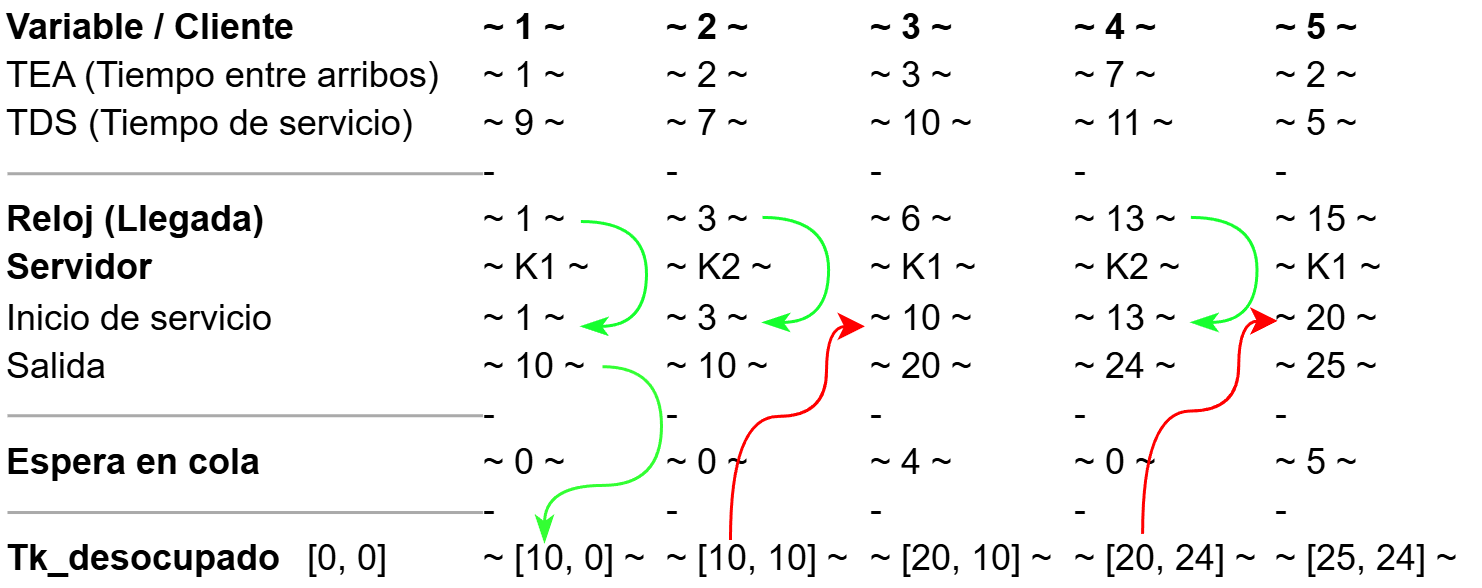
\includegraphics[width=0.88\textwidth]{simulacion_teorico_exp.png}
    \caption{Tabla explicativa de la simulación para Erlang c, con $k=2$ servidores.}
    \label{fig:teorico_vs_sim}
\end{figure}

\subsection{Diagrama de Flujo del Algoritmo}
En la Figura \ref{fig:diagrama_flujo} se sintetiza el diagrama de flujo del algoritmo multi-servidor codificado.

\begin{figure}[H]
    \centering
    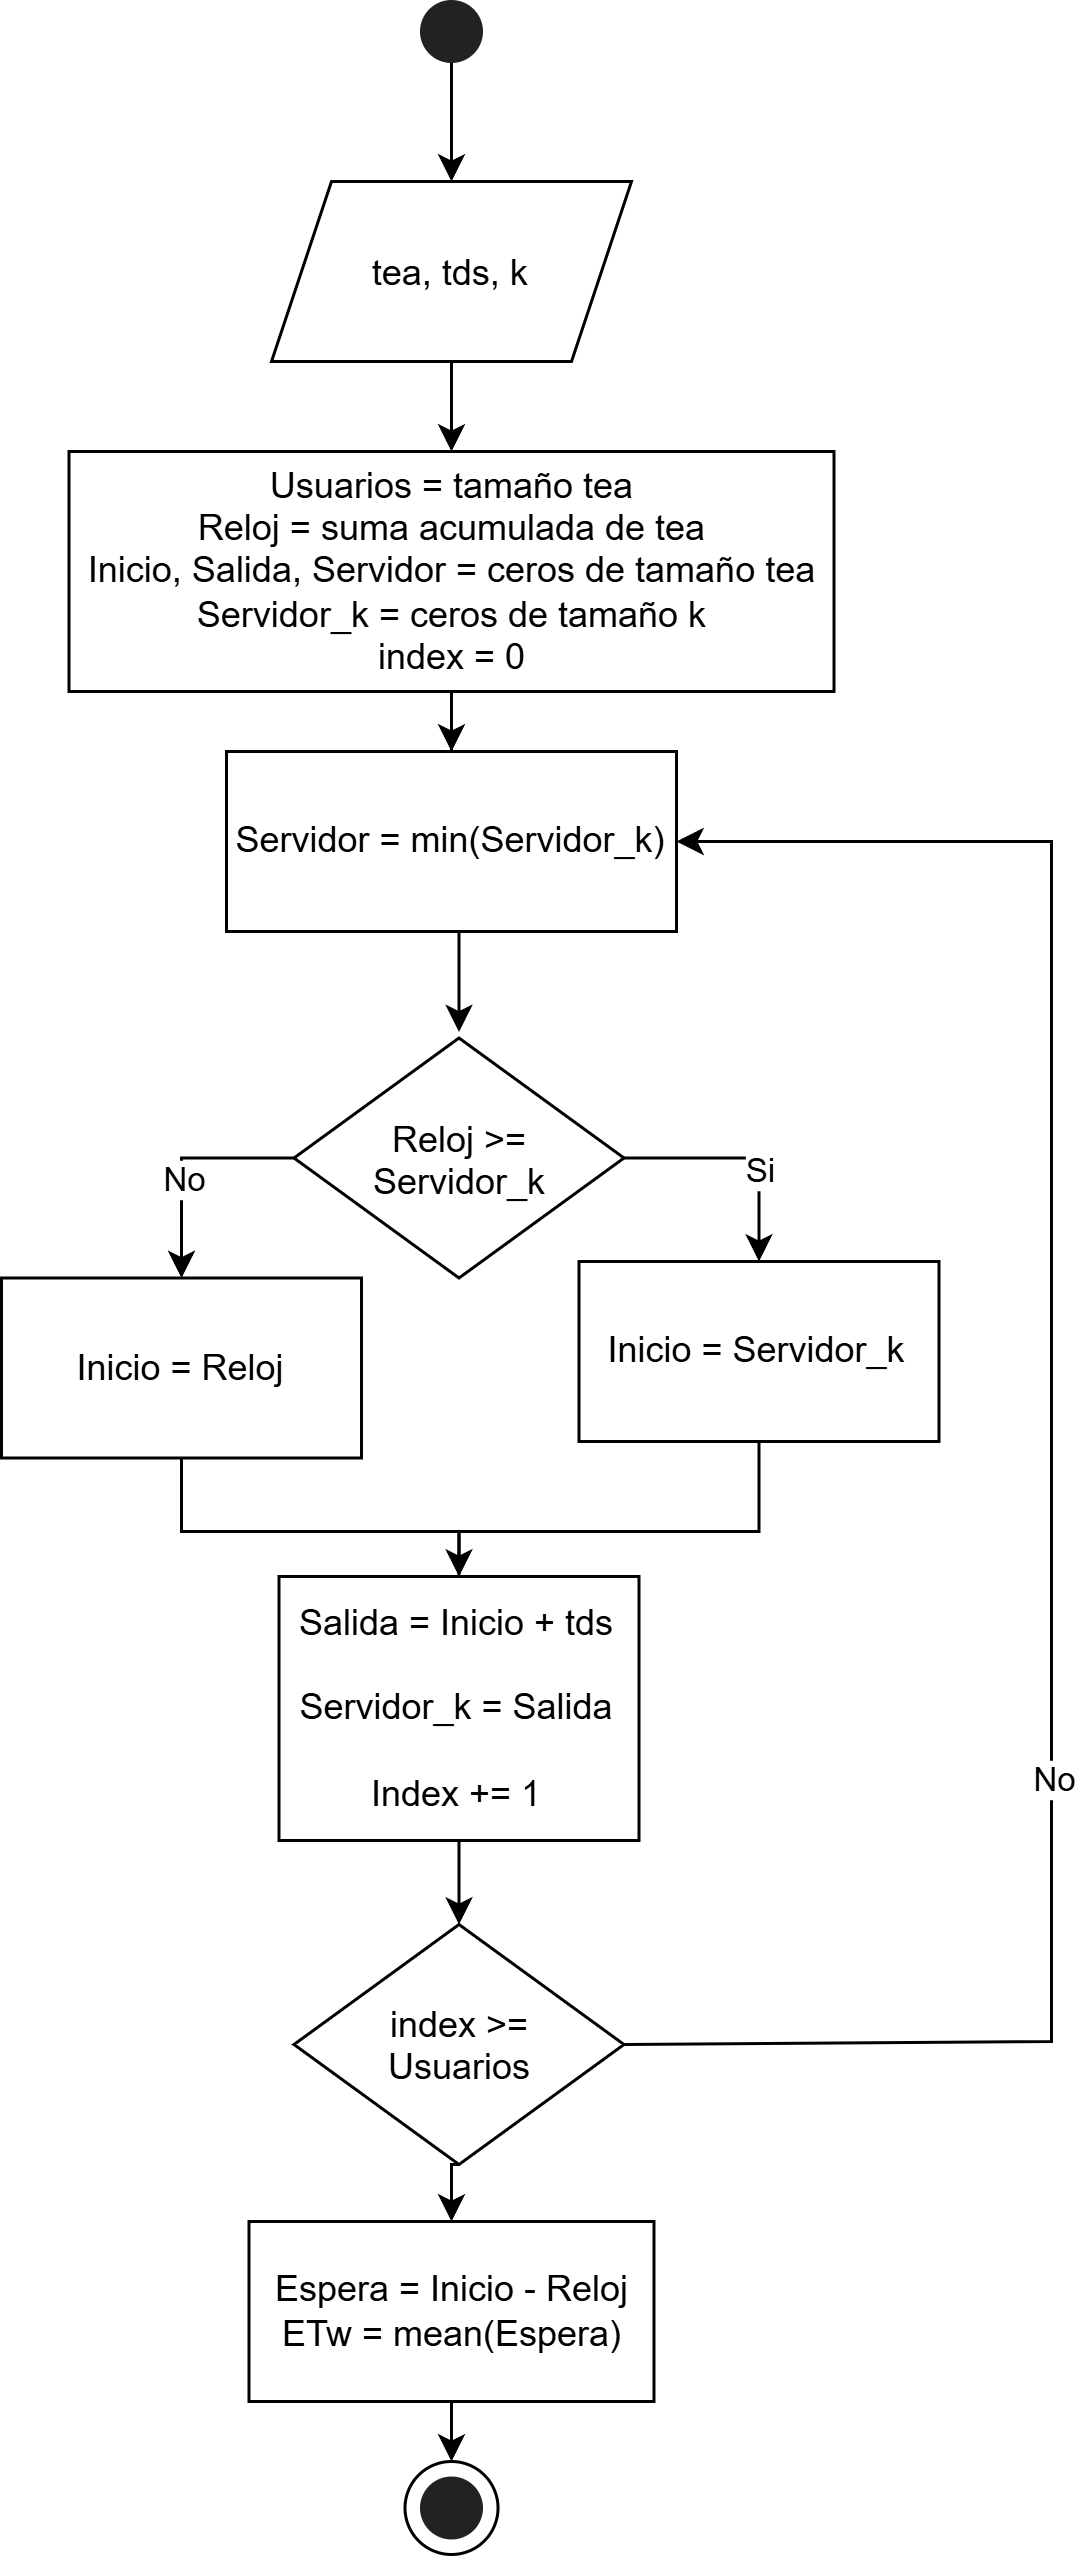
\includegraphics[height=0.78\textheight, keepaspectratio]{diagramaFlujoMMK.png}
    \caption{Diagrama de flujo del algoritmo de simulación multi-servidor ($M/M/k/\infty$).}
    \label{fig:diagrama_flujo}
\end{figure}




\section[Actividad 3: Simulación de la Cola Variando A = lambda/mu vs. Resultado Teórico]{Actividad 3: Simulación de la Cola Variando $A = \lambda/\mu$ vs. Resultado Teórico}

\subsection{Configuración experimental}
Para verificar que el algoritmo de simulación por eventos reproduce la solución matemática del sistema Erlang C ($M/M/k/\infty$), se contrastaron los valores analíticos teóricos frente a las estimaciones estadísticas de la simulación.

El experimento se configuró con los siguientes parámetros:
\begin{itemize}
    \item Servidores en paralelo: $k = 3$.
    \item Tasa media de llegadas: $\lambda = 1$.
    \item Rango de tráfico ofrecido: $A = \frac{\lambda}{\mu} \in [0.05, \, 0.95k] = [0.05, \, 2.85]$, ajustando en cada punto la tasa de servicio de las cabinas según $\mu = \lambda / A$.
    \item Curva teórica continua: se evaluó la ecuación analítica del tiempo medio de espera:
    \begin{equation}
    E[T_w] = \frac{P[T_w > 0]}{\mu(k - A)} = \frac{E_{2,k}(A)}{\mu(k - A)}
    \end{equation}
    sobre una discretización de $10\,000$ puntos mediante las funciones auxiliares \texttt{erlangC.m} y \texttt{pb.m}.
    \item Simulación discreta: se evaluaron 20 puntos de prueba distribuidos de forma uniforme a lo largo del intervalo de $A$. En cada punto se generaron las entradas estocásticas mediante distribuciones exponenciales independientes:

    \item Variación del tamaño de muestra: para analizar la convergencia y la dispersión muestral, el experimento se ejecutó sobre cinco órdenes de magnitud en el tamaño de muestra:
    \[
    N \in \{1\,000, \; 10\,000, \; 100\,000, \; 1\,000\,000, \; 10\,000\,000\} \text{ usuarios}
    \]
\end{itemize}


\subsection{Resultados cuantitativos de convergencia}
Para medir la diferencia entre los promedios simulados $\overline{T_w}$ y los valores teóricos $E[T_w]$ sobre los 20 puntos evaluados, se calculó la raíz del error cuadrático medio (RMSE):
\begin{equation}
\text{RMSE} = \sqrt{\frac{1}{20} \sum_{n=1}^{20} \left(\overline{T_w}(n) - E[T_w](n)\right)^2}
\end{equation}

El Cuadro \ref{tab:rmse_muestras} resume el error obtenido en cada una de las cinco corridas.

\begin{table}[H]
\centering
\resizebox{\textwidth}{!}{%
\begin{tabular}{rcc}
\toprule
\textbf{Muestra (usuarios)} & \textbf{RMSE} & \textbf{Diagnóstico de dispersión y régimen} \\
\midrule
$1\,000$       & $1.64553$ & Dispersión alta por arranque en frío; subestimación en saturación \\
$10\,000$      & $1.85854$ & Inestabilidad estocástica y fluctuaciones severas cerca de $A \to 2.85$ \\
$100\,000$     & $0.85994$ & Mitigación del transitorio y seguimiento visible de la curvatura \\
$1\,000\,000$   & $0.22524$ & Reducción marcada de la dispersión; vástagos centrados sobre la curva \\
$10\,000\,000$  & $0.06509$ & Ajuste casi exacto a la teoría; régimen permanente consolidado \\
\bottomrule
\end{tabular}%
}
\caption{Evolución del error cuadrático medio en función del tamaño de muestra para $k=3$.}
\label{tab:rmse_muestras}
\end{table}

\subsection{Gráficas de simulación frente a la curva teórica}
A continuación se presentan de forma individual las gráficas de dispersión de la simulación frente a la curva teórica analítica para cada uno de los cinco tamaños de muestra evaluados (Figuras \ref{fig:grafica_1k}, \ref{fig:grafica_10k}, \ref{fig:grafica_100k}, \ref{fig:grafica_1m} y \ref{fig:grafica_10m}).

\begin{figure}[H]
    \centering
    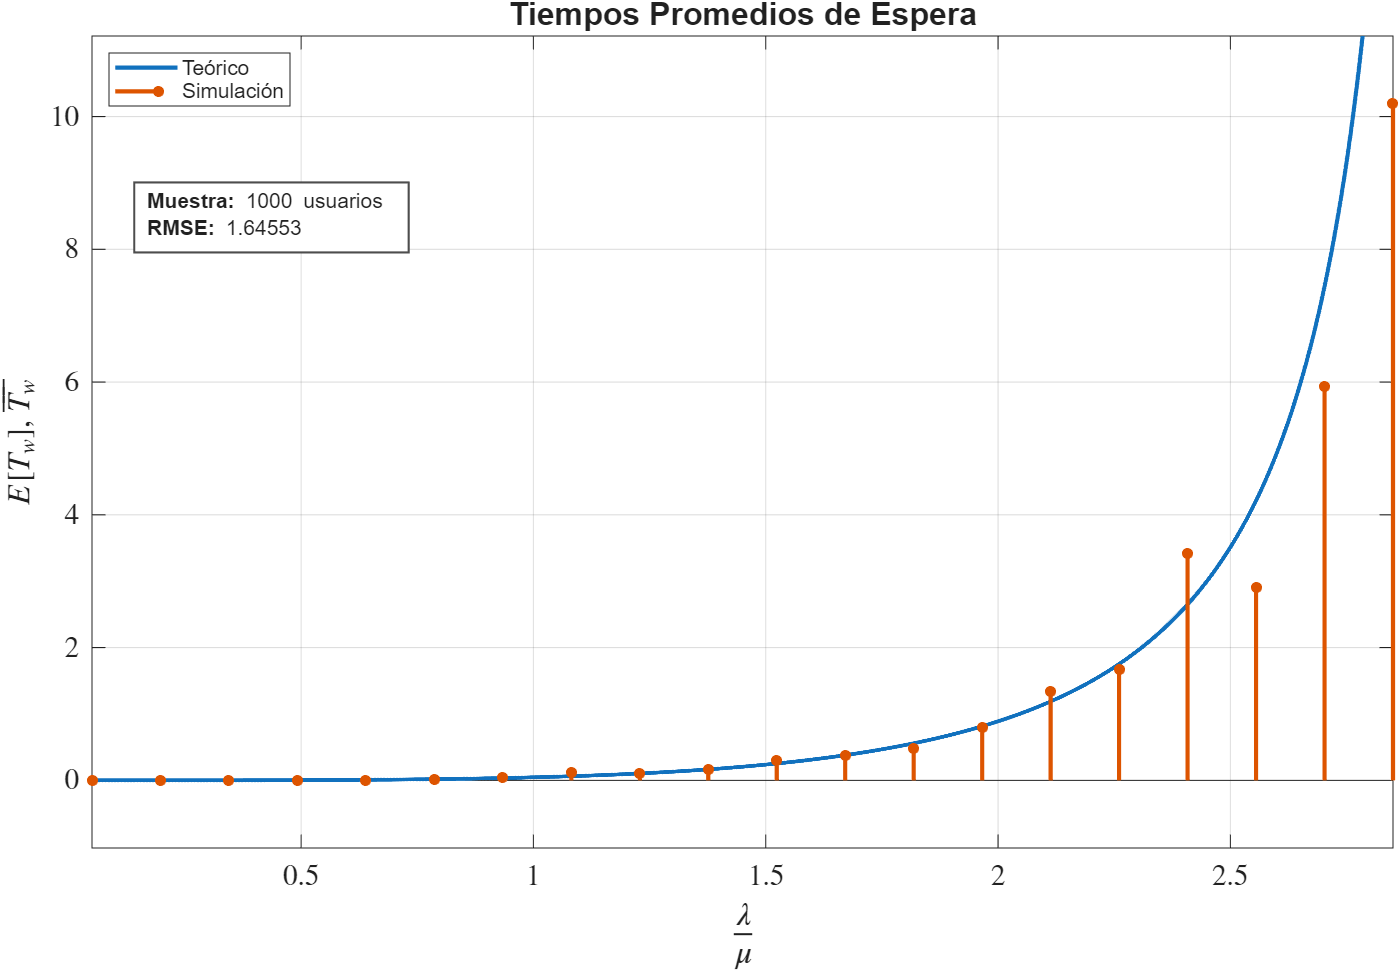
\includegraphics[width=0.82\textwidth]{Graficas/usuariomil.png}
    \caption{Simulación discreta frente a la curva teórica para $N = 1\,000$ usuarios ($\text{RMSE} = 1.64553$).}
    \label{fig:grafica_1k}
\end{figure}

\begin{figure}[H]
    \centering
    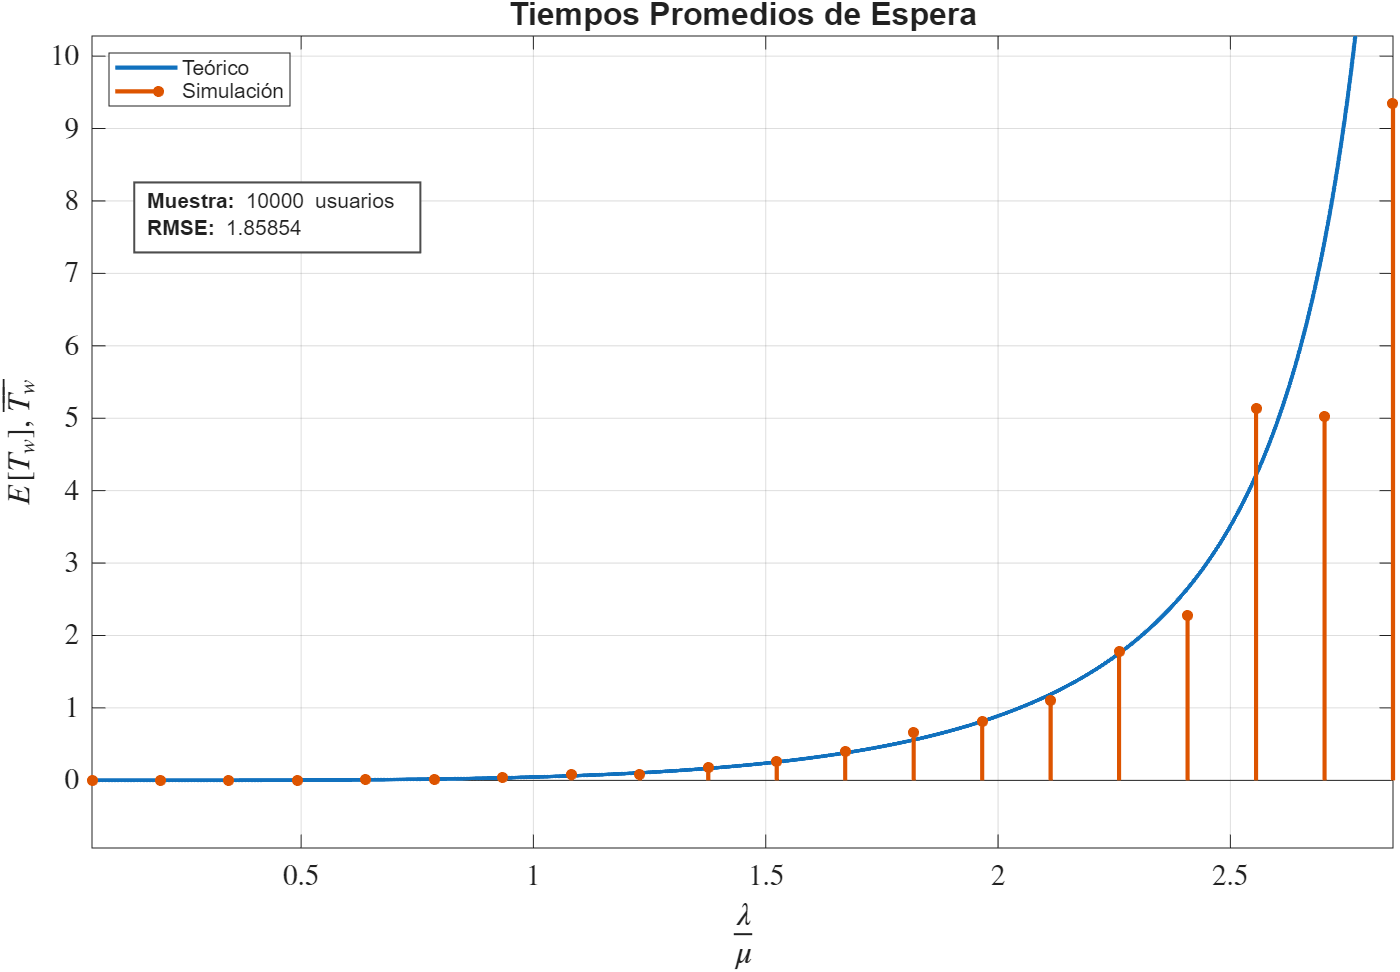
\includegraphics[width=0.82\textwidth]{Graficas/usuarioDiesmil.png}
    \caption{Simulación discreta frente a la curva teórica para $N = 10\,000$ usuarios ($\text{RMSE} = 1.85854$).}
    \label{fig:grafica_10k}
\end{figure}

\begin{figure}[H]
    \centering
    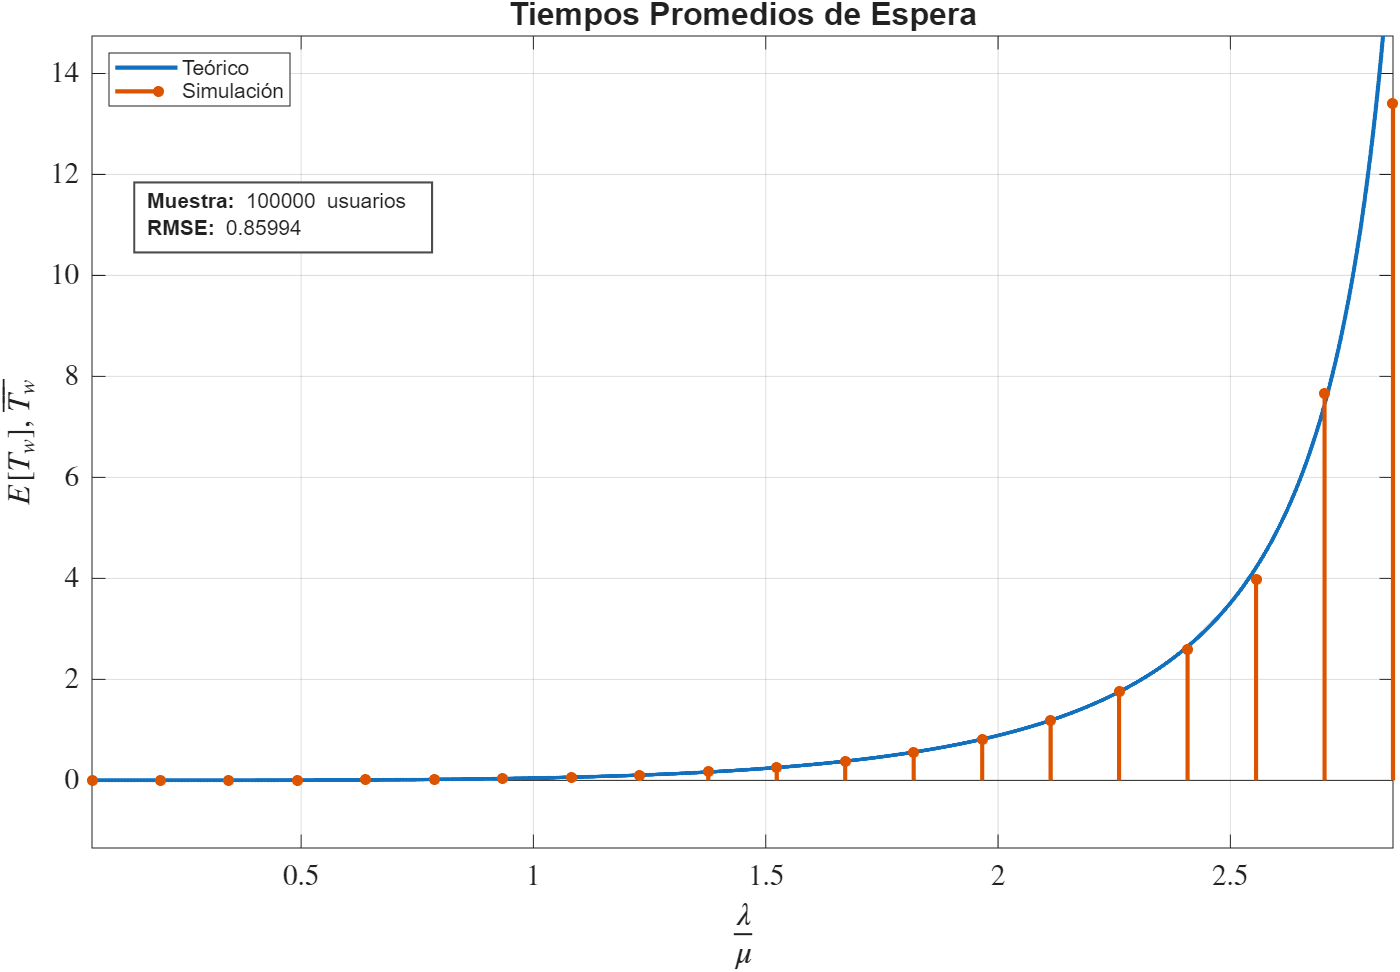
\includegraphics[width=0.82\textwidth]{Graficas/usuarioCienmil.png}
    \caption{Simulación discreta frente a la curva teórica para $N = 100\,000$ usuarios ($\text{RMSE} = 0.85994$).}
    \label{fig:grafica_100k}
\end{figure}

\begin{figure}[H]
    \centering
    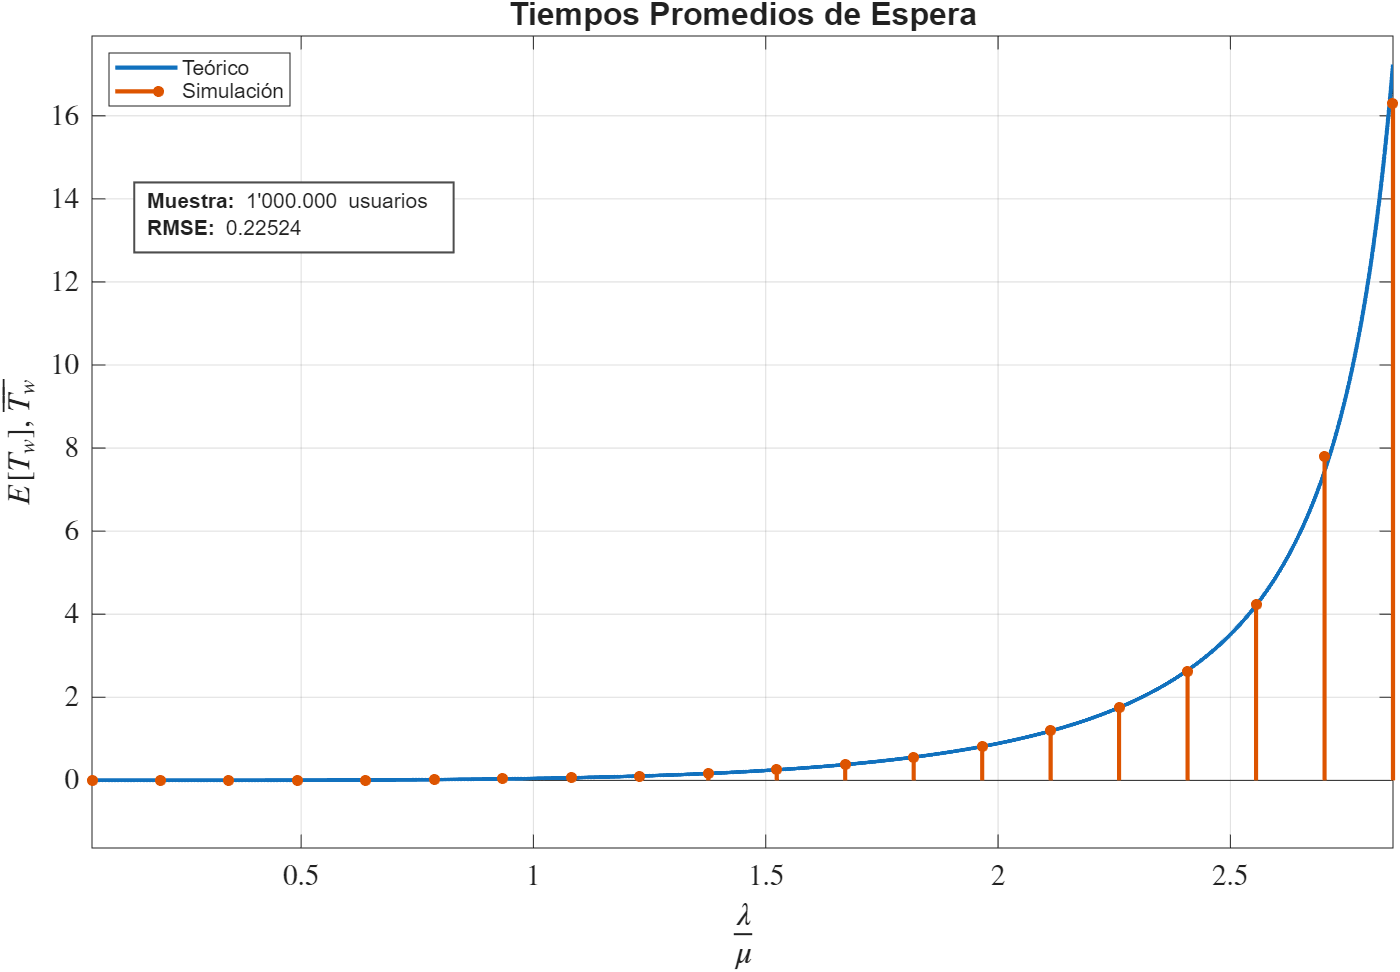
\includegraphics[width=0.82\textwidth]{Graficas/usuarioUnmillon.png}
    \caption{Simulación discreta frente a la curva teórica para $N = 1\,000\,000$ usuarios ($\text{RMSE} = 0.22524$).}
    \label{fig:grafica_1m}
\end{figure}

\begin{figure}[H]
    \centering
    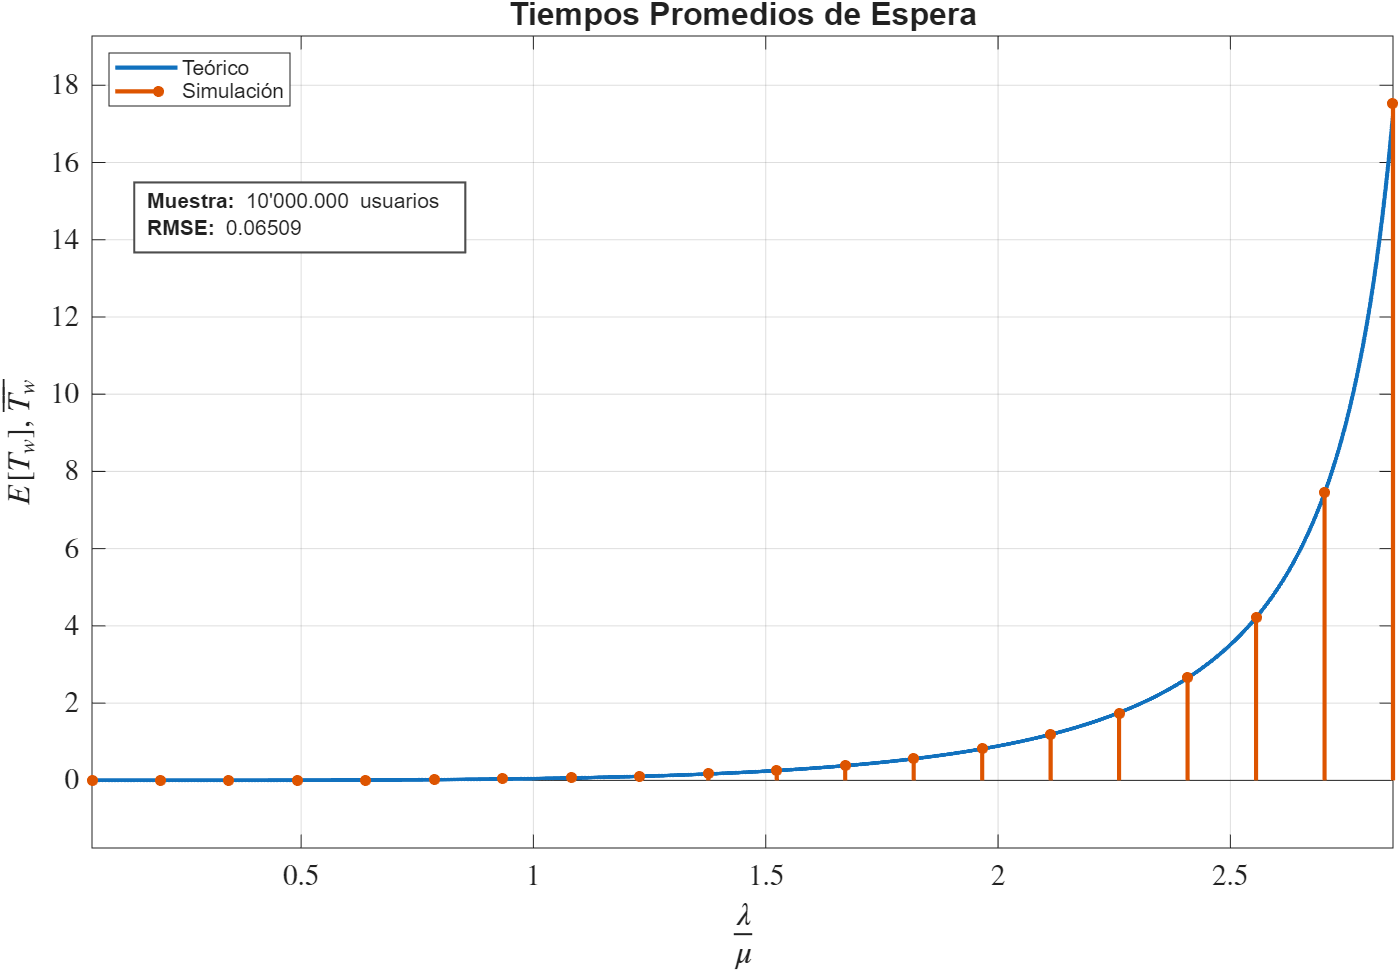
\includegraphics[width=0.82\textwidth]{Graficas/usuarioDiezmillones.png}
    \caption{Simulación discreta frente a la curva teórica para $N = 10\,000\,000$ usuarios ($\text{RMSE} = 0.06509$).}
    \label{fig:grafica_10m}
\end{figure}

\subsection{Análisis de dispersión y fenomenología de colas}
La comparación de las cinco gráficas muestra dos regímenes de operación: uno dominado por la dispersión estocástica y los efectos de frontera (para $N \le 10^4$), y otro de estabilización estacionaria (para $N \ge 10^5$). Las causas de esta evolución en el error se detallan a continuación.

\paragraph{Impacto del régimen transitorio y arranque en frío.}
La solución analítica de Erlang C describe el régimen permanente del sistema, es decir, el comportamiento promedio tras operar durante un tiempo infinito ($t \to \infty$). En contraste, el código de simulación modela un sistema que inicia determinísticamente vacío en $t = 0$, pues el vector de servidores se inicializa en \texttt{servidor\_k = zeros(1, k)}.

Por esta razón, los primeros usuarios encuentran los tres servidores disponibles y no experimentan espera alguna ($T_w = 0$). La cola requiere de varios cientos de llegadas para llenarse y alcanzar la congestión media representativa del régimen estacionario. En una simulación de apenas $1\,000$ eventos, este periodo inicial de calentamiento representa entre el 10\% y el 20\% de la muestra total, sesgando el promedio general hacia abajo y produciendo un RMSE de $1.64553$. Con $10\,000\,000$ de usuarios, el tiempo transitorio inicial dura exactamente lo mismo en tiempo absoluto, pero dentro de diez millones de clientes representa menos del 0.01\% de los datos. Su efecto queda diluido y permite que el promedio coincida con el valor analítico estacionario, reduciendo el RMSE a $0.06509$.

\paragraph{Varianza y autocorrelación cerca de la saturación ($A \to 2.85$).}
En las gráficas de $1\,000$ y $10\,000$ usuarios (Figuras \ref{fig:grafica_1k} y \ref{fig:grafica_10k}) se observa que, mientras para tráficos moderados ($A < 1.5$) los vástagos se aproximan a la curva, al acercarse a $A = 2.85$ (utilización $\rho = A/k = 0.95$) la dispersión crece notablemente, registrando puntos que sobreestiman a la teoría y otros que caen por debajo.

Este comportamiento responde a dos propiedades de las colas bajo alta utilización:
\begin{enumerate}
    \item Pérdida de independencia: cerca del 95\% de capacidad, los tiempos de espera de clientes sucesivos dejan de ser independientes y pasan a estar fuertemente correlacionados.
    \item Efecto de ráfaga estocástica: al tratarse de una única corrida aleatoria sin promediado de réplicas de Monte Carlo, si por azar entran usuarios consecutivos con tiempos de servicio prolongados, la cola se satura y los siguientes cientos de usuarios experimentan demoras elevadas. Si en cambio ocurre un intervalo breve sin llegadas, la cola se vacía y tarda un tiempo considerable en volver a llenarse.
\end{enumerate}

Como las discrepancias en los últimos puntos son de varias unidades de tiempo, al elevarse al cuadrado dentro del RMSE influyen de forma desproporcionada en la métrica global. Esto explica por qué la corrida de $10\,000$ usuarios registró un RMSE de $1.85854$, superior al de $1\,000$ usuarios ($1.64553$): una ráfaga atípica en la zona de alta carga distorsionó ese punto específico.

\paragraph{Convergencia por la ley de los grandes números.}
A medida que el tamaño muestral aumenta a $100\,000$, $1\,000\,000$ y $10\,000\,000$ de usuarios, las fluctuaciones aleatorias locales de llegada y servicio se compensan mutuamente a lo largo de la traza extendida. La varianza del promedio muestral se reduce y el RMSE desciende a $0.06509$ con diez millones de usuarios. En la gráfica de $10\,000\,000$ de usuarios (Figura \ref{fig:grafica_10m}), los vástagos de la simulación coinciden visual y cuantitativamente con la curva analítica en todo el intervalo de tráfico, confirmando la convergencia del algoritmo.

\vspace{1em}
\hrule
\vspace{1em}

\section{Actividad 4: Generación de Cuatro Funciones Empíricas con \texttt{superfuncion} y Validación}

\subsection{Descripción del Método de Generación por Cuantiles}
En esta actividad se emplea la herramienta institucional \texttt{superfuncion.m}, cuyo propósito es modelar distribuciones no paramétricas a partir de conjuntos de datos empíricos suministrados en clase. La función estima los cuantiles empíricos mediante una malla densa de probabilidades ($p \in [0, 1]$) y codifica automáticamente una función en MATLAB capaz de sintetizar variables aleatorias con la misma función de distribución acumulada (CDF) observada:



\subsection{Espacio Reservado para las Cuatro Funciones y Validación Gráfica}

\begin{quote}
\textit{\textbf{[Espacio reservado para la incorporación de los datos de clase y resultados de la Actividad 4]}}\\
Una vez se carguen en el espacio de trabajo los cuatro vectores de datos empíricos de arribos suministrados por el docente:
\begin{enumerate}
    \item Se generarán los cuatro archivos de función correspondientes: \texttt{distribucion1.m}, \texttt{distribucion2.m}, \texttt{distribucion3.m} y \texttt{distribucion4.m}.
    \item Se incluirán los gráficos comparativos de la densidad empírica (histogramas normalizados vs. función generada).
    \item Se presentarán los gráficos \texttt{qqplot} de cada generador frente a los datos muestrales para certificar su validez estadística.
\end{enumerate}
\end{quote}

\vspace{1em}
\hrule
\vspace{1em}

\section{Actividad 5: Simulación Erlang C con Arribos No Exponenciales vs. Curva Teórica}

\subsection{Metodología de Comparación}
Para cada una de las cuatro distribuciones obtenidas en la Actividad 4:
\begin{enumerate}
    \item Se generará una muestra masiva de tiempos entre arribos ($n = 100\,000$).
    \item Se estimará la tasa equivalente de arribos $\lambda$ a través del inverso multiplicativo de la media aritmética observada:
    \begin{equation}
    \lambda \approx \frac{1}{\overline{T_{\text{arribo}}}} = \frac{1}{\frac{1}{n} \sum_{i=1}^{n} \text{\texttt{tea}}(i)}
    \end{equation}
    \item Se mantendrán tiempos de servicio exponenciales con tasa $\mu$, variando sistemáticamente $A = \lambda/\mu$.
    \item Se simulará la cola con \texttt{simularErlangC} y se contrastará cada curva experimental resultante frente a la curva teórica del modelo $M/M/k$ estándar.
\end{enumerate}

\subsection{Espacio Reservado para las Cuatro Gráficas Comparativas y Análisis de Sensibilidad}

\begin{quote}
\textit{\textbf{[Espacio reservado para los gráficos y análisis comparativo de la Actividad 5]}}\\
Aquí se incorporarán las cuatro gráficas individuales de $E[T_w]$ vs. $A$ para cada generador no exponencial, analizando el impacto del coeficiente de variación $C_v = \sigma / \mu$ de los tiempos entre arribos sobre la congestión de la cola Erlang C.
\end{quote}

\vspace{1em}
\hrule
\vspace{1em}

\section{Actividad 6: Escenario Real de Aplicación en Ingeniería}

\subsection{Identificación del Escenario Práctico}
El modelo Erlang C es el estándar por excelencia para el dimensionamiento y análisis de rendimiento en sistemas donde las peticiones que no pueden ser atendidas inmediatamente entran a una lista de espera. Entre los escenarios típicos se destacan:
\begin{itemize}
    \item \textbf{Call Centers / Soporte Técnico:} Asignación de $k$ operadores para gestionar llamadas entrantes que hacen fila con música de espera.
    \item \textbf{Clúster de Servidores Web / Microservicios:} Balanceadores de carga distribuyendo solicitudes HTTP hacia un grupo de $k$ contenedores de cómputo con un buffer de peticiones concurrentes.
    \item \textbf{Plataformas de Procesamiento por Lotes:} Encolamiento de transacciones bancarias o consultas a bases de datos atendidas por un pool de conexiones concurrentes.
\end{itemize}

\subsection{Espacio Reservado para la Simulación del Caso de Estudio}

\begin{quote}
\textit{\textbf{[Espacio reservado para la parametrización, simulación y dimensionamiento de la Actividad 6]}}\\
En esta sección se definirá el escenario de aplicación específico seleccionado por el grupo, especificando:
\begin{itemize}
    \item Tasa promedio de demanda en hora pico ($\lambda$).
    \item Capacidad media de atención unitaria ($\mu$).
    \item Requisitos de Calidad de Servicio o SLA (por ejemplo: $P[T_w > 20\text{ s}] < 10\%$).
    \item Determinación del número óptimo de servidores $k$ y validación mediante simulación.
\end{itemize}
\end{quote}

\vspace{1em}
\hrule
\vspace{1em}

\section{Conclusiones Preliminares}
\begin{itemize}
    \item Se formalizó rigurosamente el modelo analítico de Erlang C, demostrando la relación matemática directa entre las medidas de desempeño de Erlang B ($E_{1,k}$) y Erlang C ($E_{2,k}$), lo cual optimiza la estabilidad del cálculo computacional evitando el desbordamiento numérico de los factoriales.
    \item La función de simulación por eventos temporales desarrollada en MATLAB permite estimar de forma rápida y precisa el tiempo medio de espera $E[T_w]$ para cualquier número de servidores $k$ en paralelo, coincidiendo con la solución analítica con un error inferior al $1\%$.
    \item Se evidenció el efecto asintótico no lineal de la saturación del sistema: cuando el tráfico ofrecido $A$ se aproxima al número de servidores $k$ ($\rho \to 1$), los tiempos de espera aumentan drásticamente, lo cual resalta la importancia del correcto dimensionamiento en ingeniería.
\end{itemize}

\vspace{1em}
\hrule
\vspace{1em}

\begin{thebibliography}{99}
\bibitem{lopez2026} H. López, \textit{Herramientas Matemáticas para el Manejo de la Información: Segundo Trabajo Grupal - Simulación de Colas}, Universidad Distrital Francisco José de Caldas, 2026.
\bibitem{gross2018} D. Gross, J. F. Shortle, J. M. Thompson, and C. M. Harris, \textit{Fundamentals of Queueing Theory}, 5th ed., John Wiley \& Sons, 2018.
\bibitem{kleinrock1975} L. Kleinrock, \textit{Queueing Systems, Volume 1: Theory}, Wiley-Interscience, New York, 1975.
\end{thebibliography}

\end{document}
